%%----------- 格式控制 ----------- %%
\documentclass[12pt, a4paper]{article}

%%----------- 引入宏包 ----------- %%
\usepackage[numbers]{gbt7714}
\usepackage[heading]{ctex}
\usepackage{xeCJK}
\usepackage[hidelinks]{hyperref}
\usepackage[final]{pdfpages}
\usepackage{natbib}
\usepackage{booktabs}
\usepackage{tabularx}
\usepackage{multirow}
\usepackage{graphicx}
\usepackage{amsmath}
\usepackage{geometry}
\usepackage{setspace}
\usepackage{fontspec}
\usepackage{fancyhdr}
\usepackage{caption}
\usepackage{titletoc}
\usepackage{titlesec}
\usepackage{amssymb}
\usepackage{siunitx}

%%----------- 页面设置 ----------- %%
\geometry{left=2.5cm, right=2.5cm, top=3cm, bottom=3cm}
\setlength{\baselineskip}{20pt}
\setlength{\headheight}{15pt}

%%----------- 字体设置 ----------- %%
\setmainfont{Times New Roman}
\newCJKfontfamily{\cusong}[AutoFakeBold={2.17}]{SimSun} % 本地编译粗宋体
\setCJKfamilyfont{song}{SimSun}
\setCJKfamilyfont{hei}{黑体\-简.TTF}

%%----------- 目录设置 ----------- %%
\titlecontents{section}[0pt]{\addvspace{0pt}\filright}
{\contentspush{\thecontentslabel\ \ }}
{}{\titlerule*[4pt]{.}\contentspage}

\titlecontents{subsection}[1.7em]{\addvspace{0pt}\filright}
{\contentspush{\thecontentslabel\ \ }}
{}{\titlerule*[4pt]{.}\contentspage}

\titlecontents{subsubsection}[3em]{\addvspace{0pt}\filright}
{\contentspush{\thecontentslabel\ \ }}
{}{\titlerule*[4pt]{.}\contentspage}

\titlecontents{figure}[0pt]{\addvspace{0pt}\filright}
{\figurename~\thecontentslabel\ \ }{}{\titlerule*[4pt]{.}\contentspage}

\titlecontents{table}[0pt]{\addvspace{0pt}\filright}
{\tablename~\thecontentslabel\ \ }{}{\titlerule*[4pt]{.}\contentspage}

\renewcommand{\listfigurename}{图目录}
\renewcommand{\listtablename}{表目录}
\setcounter{secnumdepth}{4}

%%----------- 标题设置 ----------- %%
\titleformat{\section}{\centering\bfseries\heiti\zihao{3}}{\thesection}{1em}{\heiti\zihao{3}}
\titleformat{\subsection}{\bfseries\heiti\zihao{4}}{{\thesubsection}}{0.5em}{\heiti\zihao{4}}
\titleformat{\subsubsection}{\bfseries\heiti\zihao{-4}}{{\thesubsubsection}}{0.5em}{\heiti\zihao{-4}}
\titleformat{\paragraph}[hang]{\zihao{-4}}{\theparagraph}{0.5em}{\zihao{-4}}

\titlespacing{\section}{6pt}{*2}{*2}
\titlespacing{\subsection}{0pt}{4pt}{6pt}
\titlespacing{\subsubsection}{0pt}{6pt}{6pt}
\titlespacing{\paragraph}{0pt}{6pt}{6pt}

%%----------- 编号设置 ----------- %%
\renewcommand{\thesection}{第\arabic{section}章}
\renewcommand{\thesubsection}{\arabic{section}.\arabic{subsection}}
\renewcommand{\thesubsubsection}{\arabic{section}.\arabic{subsection}.\arabic{subsubsection}}
\renewcommand{\theparagraph}{\arabic{section}.\arabic{subsection}.\arabic{subsubsection}.\arabic{paragraph}}

\counterwithin{figure}{section}
\counterwithin{equation}{section}
\counterwithin{table}{section}
\renewcommand{\theequation}{\arabic{section}.\arabic{equation}}
\renewcommand{\thefigure}{\arabic{section}.\arabic{figure}}
\renewcommand{\thetable}{\arabic{section}.\arabic{table}}
\renewcommand{\figureautorefname}{图}
\renewcommand{\tableautorefname}{表}
\renewcommand{\arraystretch}{1.3}

\renewcommand{\headrulewidth}{0.05mm}

%%----------- 参考文献设置 ----------- %%
\renewcommand\refname{参考文献}
\setlength{\bibsep}{0pt}
\setcitestyle{super}
\newcommand{\upcite}[1]{\textsuperscript{\textsuperscript{\cite{#1}}}}

%%----------- Caption设置 ----------- %%
\captionsetup[figure]{aboveskip=6pt, labelformat=default, labelsep=space, font=small}
\captionsetup[table]{belowskip=12pt, aboveskip=6pt, labelformat=default, labelsep=space, font=small}

\begin{document}

%%----------- 前言部分 ----------- %%
\newgeometry{left=2.54cm, right=2.54cm, top=3.18cm, bottom=3.18cm}
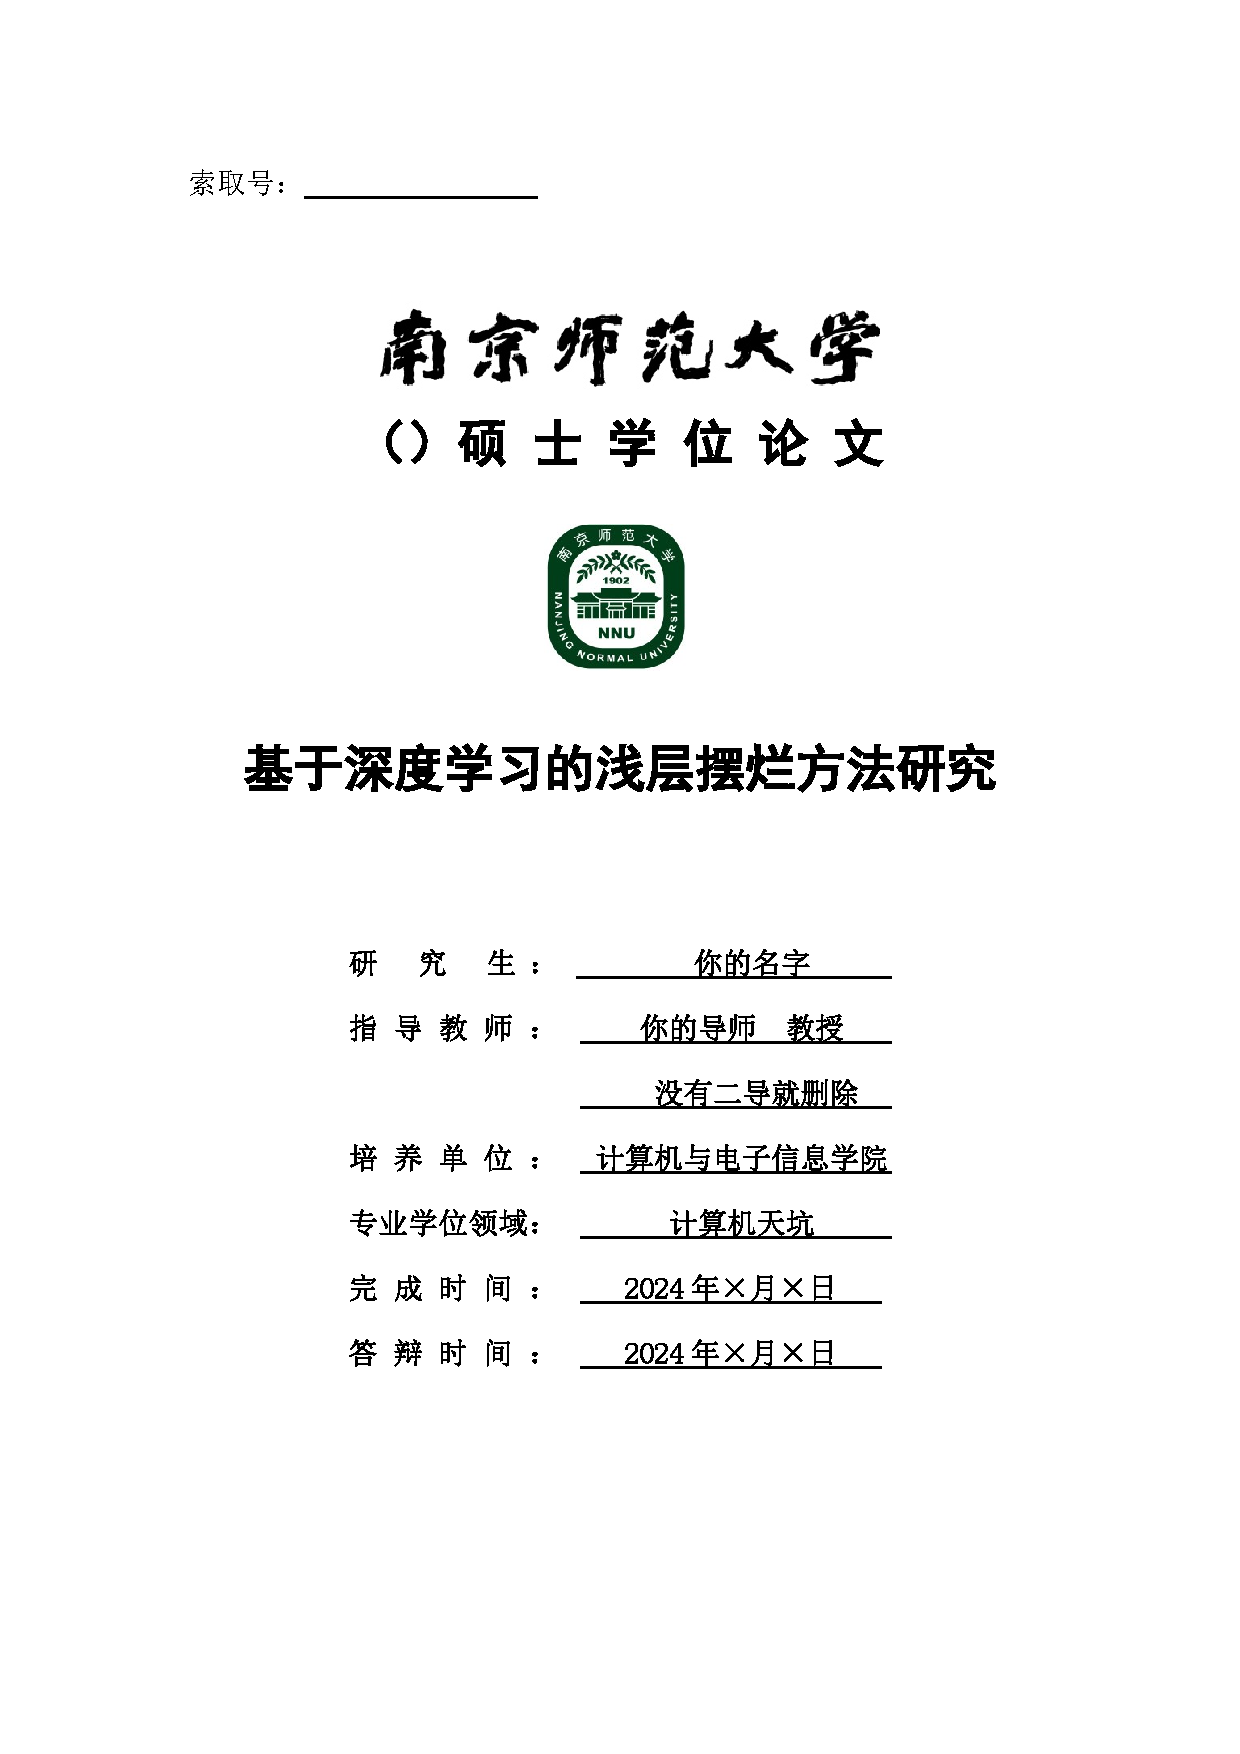
\includepdf{cover/cover.pdf} % 封面文件
%中英文摘要

{\centering\section*{摘 \quad 要}}
\phantomsection
\addcontentsline{toc}{section}{摘\hspace{1em}要}
\pagestyle{fancy}
\fancyhf{}
\fancyfoot[CO, CE]{\thepage} % 页脚页码信息
\pagenumbering{Roman}	%定义字体
\fancyhead[C]{摘要} % 页眉信息
%此处开始写中文摘要
本模板出自计算机学院自然语言处理实验室的前辈们,适用于南京师范大学硕士毕业论文理工科类,仅作为参考使用,后续可根据具体的要求变动进行修改,最后一次更新于2024年3月份。

模板由地理科学学院卫星定位与导航课题组修改,最后一次修改于2024年7月。

如果你发现了问题,请修改然后上传,为学弟学妹们节省宝贵的修改word格式的时间,祝大家毕业顺利!


\par\noindent\textbf{关键词}:南师大,计算机

\newpage %分页
{\centering\section*{Abstract}} 
\phantomsection
\addcontentsline{toc}{section}{Abstract}%把摘要添加到目录列表中,以section级别出现。
\fancyhead[C]{Abstract} 

%此处开始写英文摘要

This is an unofficial \LaTeX{} template from Computer Science College NLP LAB, and some mistakes may occur during your writing. 

Modified by School of Geodesy GNSS Team at July 2024.

Please make sure you are under correct operations when using it. If you find something wrong or items to update, renew this template and upload to the overleaf, thanks for your giant cooperation, have a successful graduation, and have a good day. 

\par\noindent\textbf{Keywords}: NNU, NLP LAB, 106, GNSS, 420 % 中英文摘要

%%----------- 页眉页脚设置 ----------- %%
\restoregeometry
\newpage
\pagestyle{fancy}
\fancyhf{}
\fancyhead[CO, CE]{\leftmark}
\fancyfoot[CO, CE]{\thepage}

%%----------- 目录格式 ----------- %%
\tableofcontents
\markboth{目录}{目录}
\newpage

% 图目录,不需要可以删掉
\listoffigures
\phantomsection
\addcontentsline{toc}{section}{图目录}
\newpage

% 表目录,不需要可以删掉
\listoftables
\phantomsection
\addcontentsline{toc}{section}{表目录}
\newpage

%%----------- 主体部分 ----------- %%
\pagenumbering{arabic}
%第一章

\section{绪论}
\subsection{简单介绍}
\subsubsection{插入表格}
需要分段的文字换行两次就可以分隔开了,\LaTeX 会帮助你整理格式。

你看如果这样就能分三段了,如果需要加粗可以选中要\textbf{加粗的字},按ctrl+b快捷加粗。下划线则需要自己键入指令:\underline{下划线}。
\paragraph{使用四级标题}

\subsubsection{插入表格}
可以直接通过将图片粘贴到这里,选择上传到的文件夹,修改图片名称即可。可以直接拖拽文件到文件夹,点确定就行了,图片都会在云端存储,不用担心,也可以跨项目上传。在文中引用图片使用\ref{fig:exm}命令即可。
\begin{figure}[h]
    \centering
    
\includegraphics[width=0.3\linewidth]{figs/image.png}
    \caption{bjh好美}
    \label{fig:exm}
\end{figure}

\subsubsection{插入图表}如表\ref{tab:example}所示,表格也可以去在线生成,或者复制Excel里的格式扔给gpt啥的生成\LaTeX 代码就行。

\begin{table}[h]
\centering
\caption{示例表格}
\label{tab:example}
\renewcommand{\arraystretch}{1.3} % 设置行高为1.3倍,默认是1.0,有需要的添加上去改
\begin{tabular}{ccc}%有几个c代表有几列,c代表居中,l和r分别表示靠左或靠右。
\toprule
列1 & 列2 & 列3 \\%每列的数据由&分隔。
\midrule
数据1 & 数据2 & 数据3 \\
数据4 & 数据5 & 数据6 \\
\bottomrule
\end{tabular}
\end{table}

\subsubsection{插入公式}公式如果带编号则需要包裹在下面的环境中,\LaTeX 公式编辑建议去网上搜在线的生成器,或者Axmath这种软件,很方便的,但用熟练的话就能自己打了,我随便打一个吧。
\begin{equation}
    X\left[ k \right] =\sum_{m=0}^{M-1}{x\left[ m \right] \left( \cos \left( \frac{2\pi}{M}km \right) -\ j\sin \left( \frac{2\pi}{M}km \right) \right)},
\end{equation}
如果是多组公式的话可以用aligned包裹,或者挨个equation就行了。举个栗子,注意各个公式之间的换行符。%注意这里没和上面的公式隔开一行,所以不是新的段落,没有首行缩进字符。

\begin{equation}
    \begin{aligned}
        X\left[ k \right] =\sum_{m=0}^{M-1}{x\left[ m \right] \left( \cos \left( \frac{2\pi}{M}km \right) -\ j\sin \left( \frac{2\pi}{M}km \right) \right)},\\
        X\left[ k \right] =\sum_{m=0}^{M-1}{x\left[ m \right] \left( \cos \left( \frac{2\pi}{M}km \right) -\ j\sin \left( \frac{2\pi}{M}km \right) \right)},\\
        X\left[ k \right] =\sum_{m=0}^{M-1}{x\left[ m \right] \left( \cos \left( \frac{2\pi}{M}km \right) -\ j\sin \left( \frac{2\pi}{M}km \right) \right)},
    \end{aligned}
\end{equation}

关于正文中如果想要插入公式的话需要dollar符号包裹,比如$ conv\ 3 \times 3$,也可以用\( \),空格通常需要以$\ $形式出现。

\subsubsection{参考文献}需要去找文献的bibtex格式,把复制到paper.bib这个文件里面,然后在文中\cite{nussbaumer1982fast}即可,默认的引用就是上引,不需要再修改了。后面的参考文献也会自动生成。

\subsubsection{小标题不会自动换行}ctrl+s或者ctrl+enter进行编译,有问题就多编译几次,右边会生成pdf的预览,随时关注生成的效果。


\newpage%分页指令 % 第1章
%第二章

\section{相关研究工作}



\newpage % 第2章
%第3章

\section{总结与展望}
Anyway,如果有遇到什么问题请积极百度或者寻求帮助,用好\LaTeX。
\newpage % 第3章

%%----------- 结尾部分 ----------- %%
%附录(如有)

\clearpage
\phantomsection
\addcontentsline{toc}{section}{附录\hspace{0.5em}A}
\fancyhead[C]{附录}
{\centering\section*{附录\hspace{0.5em}A}}

在这里写附录

\newpage % 附录(如有)

\clearpage
\phantomsection
\addcontentsline{toc}{section}{参考文献} % 参考文献
\fancyhead[C]{参考文献}
\bibliography{ref/paper} % bib文件
\newpage

%在读期间发表的学术论文及研究成果

\clearpage
\phantomsection
\addcontentsline{toc}{section}{在读期间发表的学术论文及研究成果}
\fancyhead[C]{在读期间发表的学术论文及研究成果}
{\centering\section*{在读期间发表的学术论文及研究成果}}
\begin{enumerate}
    \item 写自己的研究成果,一个研究成果一个item
    \item 反正我没发
\end{enumerate}
\newpage % show time
%致谢

\clearpage
\phantomsection
\addcontentsline{toc}{section}{致\hspace{1em}谢}
\fancyhead[C]{致谢}
{\centering\section*{致 \quad 谢}}

感谢老师,感谢父母,感谢恩恩优,感谢同学,感谢CCTV。 % 致谢

\end{document}
